\documentclass[A4]{article}
\usepackage{geometry}
\geometry{verbose,tmargin=2.5cm,bmargin=2.5cm,lmargin=3cm,rmargin=3cm}
\usepackage{amsmath,amssymb,amsthm}
\usepackage{graphicx}
\graphicspath{{graphics/}}
\usepackage[utf8]{inputenc}
\usepackage{fancyvrb}
\usepackage{hyperref}
\usepackage{lscape}
\usepackage{adjustbox}
\usepackage{verbatim}

\title{MultiFEBE \\ Tutorial 1: static analysis of a plain strain elastic square with boundary elements}
\author{J.D.R. Bord\'on\\ \'A.G. Vega-Artiles}
\date{June 2022}

\begin{document}

\maketitle

\begin{figure}[h]
\centering
\includegraphics{square.eps}
\caption{Problem layout.}
\label{fig:layout}
\end{figure}

\section{Problem description}

In this first tutorial, a static analysis of a plain strain elastic square is performed using the Boundary Element Method (BEM), i.e. boundary elements. Figure \ref{fig:layout} shows the geometry, required material properties and boundary conditions, where $E$ is the Young's modulus, $\nu$ is the Poisson's ratio, $L$ is the square side length and $P$ is the load. Note that self-weight is not considered. The analytical solution to this problem is easily obtained, which results are the following displacement and stress fields:

\begin{align}
u_1 &= \dfrac{(1+\nu)(1-2\nu)}{E(1-\nu)} P x_1 \\
u_2 &= 0 \\
\sigma_{11} &= P \\
\sigma_{22} &= \dfrac{\nu}{1-\nu}P \\
\sigma_{12} &= 0
\end{align}

from which it can be checked that tractions $t_i=\sigma_{ij}n_j$ ($n_j$ are the components of the outward unit normal components) obviously verify the boundary conditions. Displacement field is linear along $x_1$-direction and constant (null) along $x_2$-direction. Also, the only non-null stresses ($\sigma_{11}$ and $\sigma_{22}$) are constant. Therefore, numerical solution using linear or higher order elements must recover the analytical solution.

The problem is solved for $L=1$ $\mathrm{m}$, $E=1$ $\mathrm{N/m^2}$, $\nu=0.25$  and $P=1$ $\mathrm{N/m^2}$ and the results are the following:

	$u_1 = 0.8\overline{3} x_1$ $\mathrm{m}$;
	$u_2 = 0$;
	$\sigma_{11} = 1$ $\mathrm{N/m^2}$;
	$\sigma_{22} = 0.\overline{3}$ $\mathrm{N/m^2}$;
	$\sigma_{12} = 0$.

\section{Preamble about the BEM and MultiFEBE}

The meshing phisolosophy is somewhat different between Boundary Element Method and the Finite Element Method (FEM). The more obvious and important difference is the fact that only the discretization of the boundary of each region\footnote{We use the term ``region'' as a synonym of ``sub-domain'', i.e. the whole problem domain is divided into one or more ``regions''.} is required, except if body loads or other special internal features are present in the problem. That is: one-dimensional (line) elements are required in two-dimensional models, and two-dimensional (surface) elements are required in three-dimensional models. Another important difference is the presence of the traction vector components as nodal degrees of freedom along with the displacement vector components. This has important implications regarding discretization, because, while the displacements field is continuous along the boundary of any given region, traction vector depends on the unit normal, which can be discontinuous. Therefore, unlike the FEM, which has an intuitive continuous volume discretization, the BEM requires taking into account additional considerations when meshing.

There are several approaches when implementing the BEM. MultiFEBE uses conventional continuous elements with multiple nodes\footnote{Multiple nodes refer to the fact that there are several nodes belonging to different elements at the same location.} where necessary, and an automatic (but configurable) collocation approach which deals with the collocation of boundary integral equations. Even though in principle it is possible to automate the process of doubling the nodes from the high-level information in the model, this responsibility is left to the user for the sake of transparency and versatility, and also because the rules governing this procedure are easy. Let $\Omega$ be a region, and $\partial\Omega$ its boundary. The boundary $\partial\Omega$ must be subdivided into a set of boundaries $\Gamma_j$ such that $\partial\Omega=\bigcup\Gamma_j$ according to the following rules:

\begin{enumerate}
    \item There must be at least a different boundary $\Gamma_j$ for each part of the boundary $\partial\Omega$ with different boundary (or interface) conditions. This is the initial obvious way of subdividing the whole boundary according to the different physics of each boundary part.
    \item Although not mandatory, it is recommended that each boundary is a connected space, i.e. each boundary is made of one monolithic piece.
    \item Each boundary $\Gamma_j$ must have unique nodes, or, in other words, each node belongs to only one boundary.
    \item Nodes must be duplicated along sharp corner and edges. 
\end{enumerate}

In summary, the user should think of the whole mesh as a set of smooth independent meshes (one per boundary).

\section{Pre-processing} 

Pre-processing in MultiFEBE consists of defining the geometry and mesh of the problem. There are three ways to do such definition: directly from the input file (mode = 0), from another file in the native format (mode = 1) or from another file in the Gmsh MSH file format version 2.2 (mode = 2), where syntax will be explained in the following subsections. Furthermore, as the problem will be solved using only the BEM formulation, the approaches explained in the previous section will be applied.      

\subsection{Gmsh format}

Gmsh \cite{gmsh, gmshweb} is a "finite element mesh generator and post-processor" with its own language. The software allows to create the geometry in a “bottom-up” manner, going from the most basic elements (points) to the highest order elements (volumes) or in a “Constructive Solid Geometry” manner (boolean operations) or with a combination of methodologies. Gmsh also allows to define  the so-called “physical groups” which are "groups of model entities" that gather elementary entities, where every entity must have a unique tag. On the other hand, the file containing all this geometric definition is the file *.geo whereas the mesh definition is in the file *.msh. 

\subsubsection{File *.geo}

The Gmsh language allows to define parameters to use later in the script and comments as every other programming language. In this example two parameters are defined: the square side length (L) and the mesh element size (es). Every point in the geometry can be specified by its coordinates (x y z) and the mesh element size to use there with the function "Point" and every straight line of the model is created with the function "Line" and its initial and final points. Then, with the function "Physical Line" every line is converted into a single entity or physical entity with its own name. Furthermore, it is worth noting that “if an expression defines a new entity, it is enclosed between parentheses but if an expression refers to a previously defined entity, it is enclosed between braces.” \cite{gmshweb} 

Finally, the mesh generation, the element order and the *.msh file saving can also be specified with the expressions \textit{Mesh + mesh dimension}, \textit{SetOrder + element order} and \textit{Save + "name.msh"}, respectively.

The resultant *.geo file applied to the problem is the following:

\begin{Verbatim}
L = 1;  // Square side length
es = 1; // Element size

// Bottom
Point (1) = {0, 0, 0, es};
Point (2) = {L, 0, 0, es};
Line (1) = {1, 2};
Physical Line ("bottom", 1) = {1};

// Right
Point (3) = {L, 0, 0, es};
Point (4) = {L, L, 0, es};
Line (2) = {3, 4};
Physical Line ("right", 2) = {2};

// Top
Point (5) = {L, L, 0, es};
Point (6) = {0, L, 0, es};
Line (3) = {5, 6};
Physical Line ("top", 3) = {3};

// Left
Point (7) = {0, L, 0, es};
Point (8) = {0, 0, 0, es};
Line (4) = {7, 8};
Physical Line ("left", 4) = {4};

// Mesh generation
Mesh 1;
SetOrder 1;
Save "t1.msh";
\end{Verbatim}

\begin{figure}[h]
	\centering
	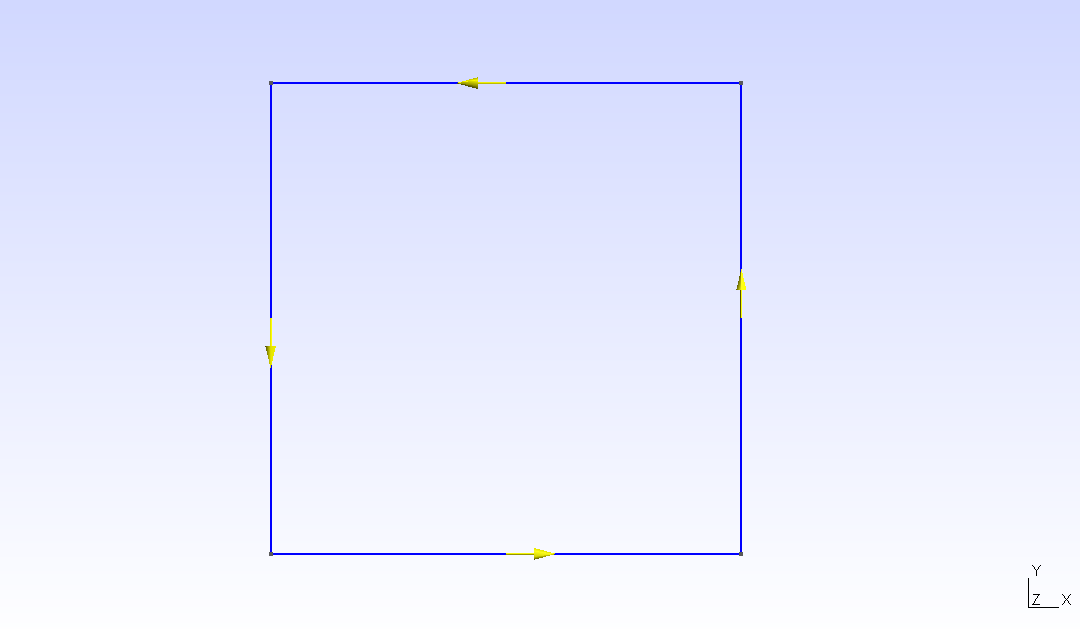
\includegraphics[scale = 0.5]{geometry2.png}
	\caption{File *.geo. Geometry with tangent vectors.}
	\label{fig:geometry}
\end{figure}

\subsubsection{File *.msh}

The *.msh file begins with a mandatory section about information of the file (MeshFormat) and following by the other sections. Here, three sections are used: the physical group names (PhysicalName), the nodes (Nodes) and the elements (Elements).

In the section "PhysicalName", all the physical entities of the model are defined. The first line
indicates the number of physical entities. Then, one line per physical entity indicating the physical dimension, the tag and the name.  
   
In the section "Nodes", all the nodes of the model are defined. The first line indicates the number of nodes. Then, one line per node indicating the identifier of the node and its coordinates (x y z).

In the section "Elements", all the elements of the model are defined. The first line indicates the number of elements. Then, one line per element indicating:

\begin{itemize}
	\item Element identifier.
	\item Type of element.
	\item Number of auxiliary tags.
	\item List of tags, where the two first auxiliary tag are mandatory, and corresponds to the identifier of the physical entity to which the element belongs and the second one is the identifier of the elementary model entity to which the element belongs. The rest of the tags are optional.
	\item A list of identifiers corresponding to the nodes of the element.
\end{itemize}

For example, in this case, an element with the identifiers 3 1 2 3 3 5 6 corresponds to:

\begin{itemize}
	\item 3: element 3.
	\item 1: type 1 (2-point line).
	\item 2: it has 2 auxiliary tags.
	\item 3: it belongs to the physical entity 3.
	\item 3: it belongs to the line 3.
	\item 5, 6: it connects the nodes 5 and 6.
\end{itemize} 

Finally, the *.msh file can be obtain in  \textit{File $\to$ Export} or by following the instructions specified in the section \textit{File *.geo}.

The resultant *.msh file applied to the problem is the following:

\begin{Verbatim}
$MeshFormat
2.2 0 8
$EndMeshFormat

$PhysicalNames
4
1 1 "bottom"
1 2 "right"
1 3 "top"
1 4 "left"
$EndPhysicalNames

$Nodes
8
1 0 0 0
2 1 0 0
3 1 0 0
4 1 1 0
5 1 1 0
6 0 1 0
7 0 1 0
8 0 0 0
$EndNodes

$Elements
4
1 1 2 1 1 1 2
2 1 2 2 2 3 4
3 1 2 3 3 5 6
4 1 2 4 4 7 8
$EndElements
\end{Verbatim}

\begin{figure}[h]
	\centering
	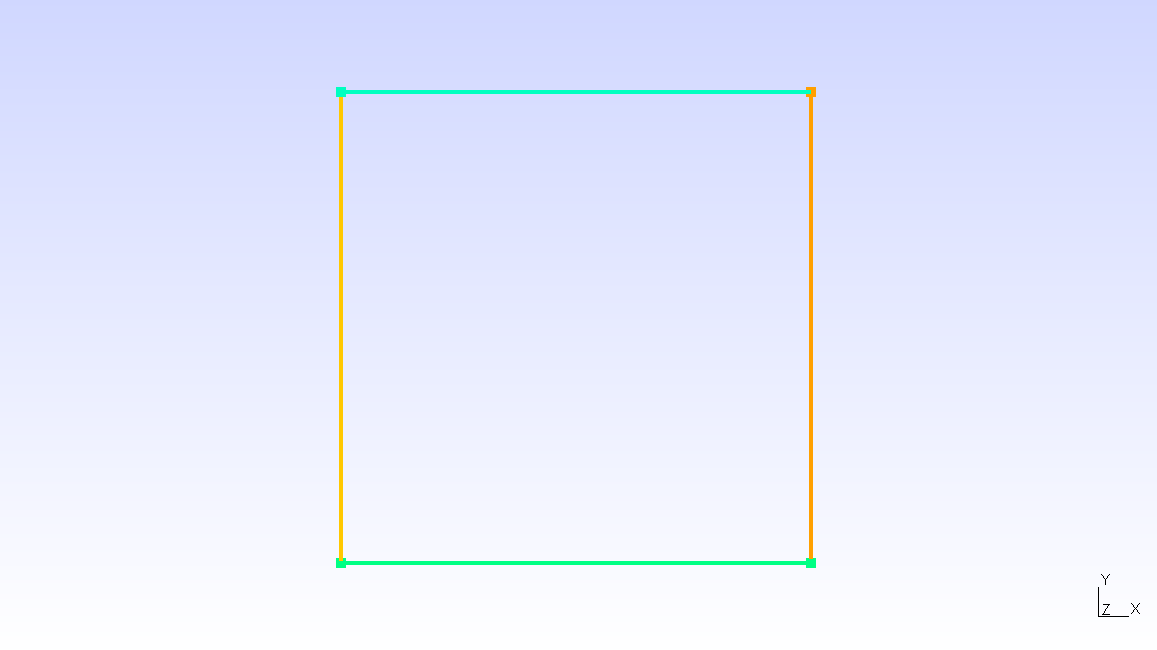
\includegraphics[scale = 0.5]{mesh.png}
	\caption{File *.msh. Mesh.}
	\label{fig:mesh}
\end{figure}

\subsection{Native format}

By default, the mesh is read from the input file by writing the sections [nodes], [elements] and [parts] in the native format as long as the user doesn't specify another option. The format of sections is very similar to the corresponding section of the Gmsh file format but here the section [parts] corresponds to the section "PhysicalName".

The native format applied to the problem is the following:

\begin{Verbatim}
[nodes]
8
1 0 0 0
2 1 0 0
3 1 0 0
4 1 1 0
5 1 1 0
6 0 1 0
7 0 1 0
8 0 0 0

[elements]
4
1 1 1 1 1 2
2 1 1 2 3 4
3 1 1 3 5 6
4 1 1 4 7 8

[parts]
4
1 1 "bottom"
1 2 "right"
1 3 "top"
1 4 "left"
\end{Verbatim}

\section{Solving}

Solving in MultiFEBE consists of running the software by specifying several options in the following sections\footnote{See reference manual.}: [problem], [settings], [materials], [boundaries], [regions], [conditions over the boundaries], etc.

The first part to configurate is the problem definition in the section [problem]. This example is a 2D static mechanical problem focused on plane strain.  

\begin{Verbatim}	
[problem]
n = 2D
type = mechanics
subtype = plane_strain
analysis = static
\end{Verbatim}

Next step is to configurate the mesh. In this case, a mesh from \textit{Gmsh} will be used so that it is necessary to write the option number 2 and the document name obtained from it in the section [settings]. However, if the mesh were going to be read from the input file, it would require to write the sections [nodes], [elements] and [parts] instead.

\begin{Verbatim}	
[settings]
mesh_file_mode = 2 "t1.msh"
\end{Verbatim}

As the problem has just one material, the section [materials] will need two lines: a first line for the number of materials in the model and a second line for the properties such as tag, name, E and $\nu$.

\begin{Verbatim}	
[materials]
1
1 elastic_solid E 1. nu 0.25
\end{Verbatim}

In the section [boundaries] it is necessary to specify the number of boundaries in the first line and a line per boundary by indicating the boundary identifier, the identifier of the part that discretize it, and finally the boundary class. In this example there are 4 boundaries: boundary 1 is the part 1 of the mesh, boundary 2 the part 2, boundary 3 the part 3 and boundary 4 the part 4 and all of them are ordinary boundaries.

\begin{Verbatim}	
[boundaries]
4
1 1 ordinary
2 2 ordinary
3 3 ordinary
4 4 ordinary
\end{Verbatim}

The format of the [regions] section consists of a first line indicating the number of regions (1). Furthermore, for each region there must be a block of data consisting of several lines of data. The first one is the region identifier and the region class (discretization method) (1 be). As the region is a BE region, then the second line indicates the number of boundaries and a list of boundaries (4 1 2 3 4). The third line defines the material (material 1). Then, for a BE region, the fourth line defines the number and a list of BE body loads (0).

\begin{Verbatim}	
[regions]
1

1 be
4 1 2 3 4
material 1
0
\end{Verbatim}

In the section [conditions over be boundaries] all boundaries will be specify in global coordinates because they are planar and their normal vectors are parallel to one of the global axes. As a 2D problem, there are two lines for every boundary: a first line for the "x" direction and the second one for the "y" direction, where the first number of every line indicates the type of condition (here 0 for displacement and 1 for traction) and the second one its value.

\begin{Verbatim}	
[conditions over be boundaries]
boundary 1: 1 0.
    	0 0.

boundary 2: 1 1.
	    1 0.

boundary 3: 1 0.
	    0 0.

boundary 4: 0 0.
	    1 0.
\end{Verbatim}

The whole script applied to the problem is the following:

\begin{Verbatim}
[problem]
n = 2D
type = mechanics
analysis = static

[settings]
mesh_file_mode = 2 "t1.msh"

[materials]
1
1 elastic_solid E 1. nu 0.25

[boundaries]
4
1 1 ordinary
2 2 ordinary
3 3 ordinary
4 4 ordinary

[regions]
1

1 be
4 1 2 3 4
material 1
0

[conditions over be boundaries]
boundary 1: 1 0.
            0 0.

boundary 2: 1 1.
            1 0.

boundary 3: 1 0.
            0 0.

boundary 4: 0 0.
            1 0.           
\end{Verbatim}

\section{Post-processing}

Post-processing in MultiFEBE consists of analysing the output files exported by the software. Output files are written according to the type of analysis and model, as well as the input file export section. By default the path and name of the output files is equal to the input file but with an additional extension. The path and name can be changed when calling the solver from the terminal as explained in the reference manual. There are three main native output files with the following additional extensions: nodal solutions (*.nso), element solutions (*.eso) and stress resultant solutions (*.tot). There is also one Gmsh output file (*.pos) which contains the case mesh and results (MSH file format version 2.2). 

For the current example, only the nodal solutions and the Gmsh output file will be explained.   

\subsection{Nodal solutions file (*.nso)}

This output file is a plain text file containing the nodal (node by node) results. The file starts with a set of header lines whose first character is "$\#$" (a comment line in GNU/Linux environments), describing the file and the meaning of the main data columns. 


\begin{Verbatim}
# Program      : multifebe
# Version      : 1.0
# File_format  : nso
# Specification: 1
# Input_file   : t1.dat
# Problem n    : 2
# Description  : 
# Timestamp    : 2022-01-16 23:38:58.324

# Columns  Description
# 1-2      Step index and value.
# 3-5      Region id, class and type.
# 6-8      (if col 4 == 1) Boundary id, class and face.
# 6-8      (if col 4 == 2) Subregion id, number of DOF and 0.
# 9-11     Node id, x1 and x2.
# >=12     Node variables. Depend on the region class and type.
\end{Verbatim}

\begin{Verbatim}
0 0.0E+0 1 1 2 1 1 1 1 0.0E+0 0.0E+0 -194.029E-9    0.000E+0  0.000E+0 -333.333E-3
0 0.0E+0 1 1 2 1 1 1 2 1.0E+0 0.0E+0  833.333E-3    0.000E+0  0.000E+0 -333.333E-3	
0 0.0E+0 1 1 2 2 1 1 3 1.0E+0 0.0E+0  833.333E-3  311.627E-9  1.000E+0    0.000E+0
0 0.0E+0 1 1 2 2 1 1 4 1.0E+0 1.0E+0  833.333E-3 -311.627E-9  1.000E+0    0.000E+0
0 0.0E+0 1 1 2 3 1 1 5 1.0E+0 1.0E+0  833.333E-3    0.000E+0  0.000E+0  333.333E-3
0 0.0E+0 1 1 2 3 1 1 6 0.0E+0 1.0E+0 -194.029E-9    0.000E+0  0.000E+0  333.333E-3
0 0.0E+0 1 1 2 4 1 1 7 0.0E+0 1.0E+0    0.000E+0 -186.443E-9 -1.000E+0    0.000E+0
0 0.0E+0 1 1 2 4 1 1 8 0.0E+0 0.0E+0    0.000E+0  186.443E-9 -1.000E+0    0.000E+0
\end{Verbatim}

In this case, node variables are the last four numbers where the displacement in x and y direction are the two first ones and the traction in x and y the remaining ones, respectively. 

\subsection{Gmsh results file (*.pos)}

The Gmsh output file (*.pos) is a plain text containing the case mesh and results which can be read by Gmsh. The structure of this file is similar to the file *.msh but with additional sections: "NodeData" and "ElementData". The section "NodeData" specifies nodal displacements and nodal traction in the following order: the number of string tags, the name of the string tag corresponding to the results, the number of real tags, the real tag (time value), the number of integer tags, the integer tags (time steps, scalar field components and number of associated nodal values) and the node numbers with their results. The section "ElementNodeData" specifies the stress tensor in the following order:
number of string tags, the name of the string tag corresponding to the results, the number of real tags, the real tag, the number of integer tags, the integer tags and the element numbers with the number of nodes per element value.

The whole file for the current example is in the online repository. However, the results for the third and fourth node will be presented here. 

\begin{Verbatim}
"Nodal displacements UX,UY (FE, BE +n)"
1 -0.19402918E-06  0.00000000E+00  0.00000000E+00
2  0.83333367E+00  0.00000000E+00  0.00000000E+00
3  0.83333322E+00  0.31162731E-06  0.00000000E+00
4  0.83333322E+00 -0.31162731E-06  0.00000000E+00
5  0.83333367E+00  0.00000000E+00  0.00000000E+00
6 -0.19402918E-06  0.00000000E+00  0.00000000E+00
7  0.00000000E+00 -0.18644328E-06  0.00000000E+00
8  0.00000000E+00  0.18644328E-06  0.00000000E+00

"Traction TX,TY (BE +n)"
1  0.00000000E+00 -0.33333307E+00  0.00000000E+00
2  0.00000000E+00 -0.33333369E+00  0.00000000E+00
3  0.10000000E+01  0.00000000E+00  0.00000000E+00
4  0.10000000E+01  0.00000000E+00  0.00000000E+00
5  0.00000000E+00  0.33333369E+00  0.00000000E+00
6  0.00000000E+00  0.33333307E+00  0.00000000E+00
7 -0.10000000E+01  0.00000000E+00  0.00000000E+00
8 -0.10000000E+01  0.00000000E+00  0.00000000E+00
\end{Verbatim}

\begin{figure}[h]
	\centering
	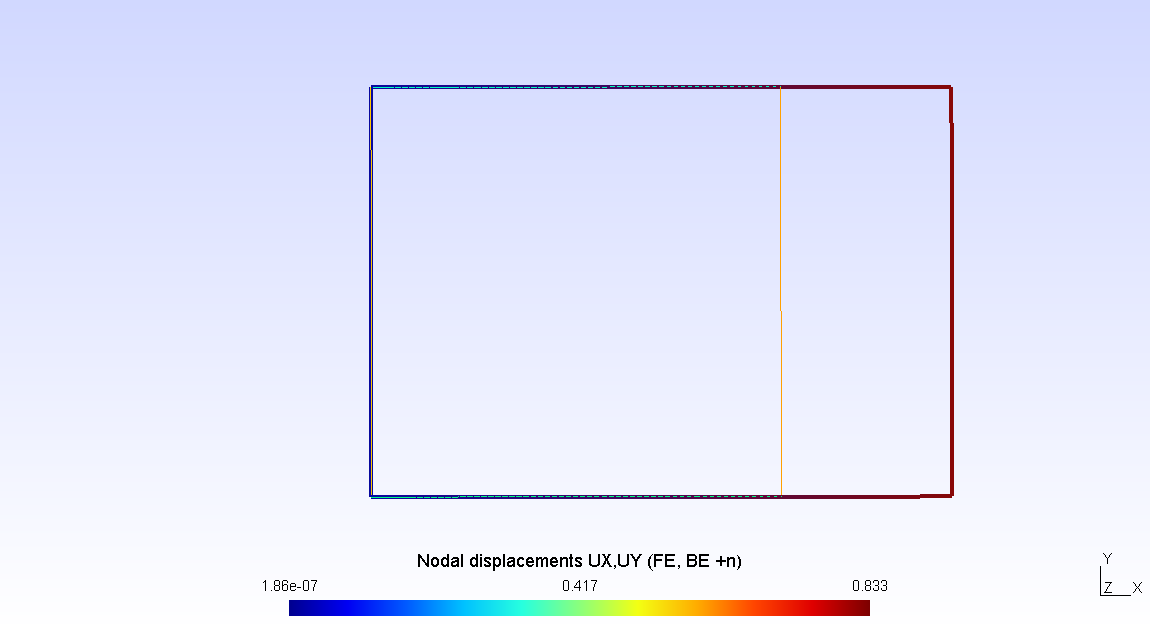
\includegraphics[scale = 0.5]{displacement.png}
	\caption{File *.pos. Nodal displacement results with a displacement factor of 0.5.}
	\label{fig:displacement}
\end{figure}

\begin{figure}
	\centering
	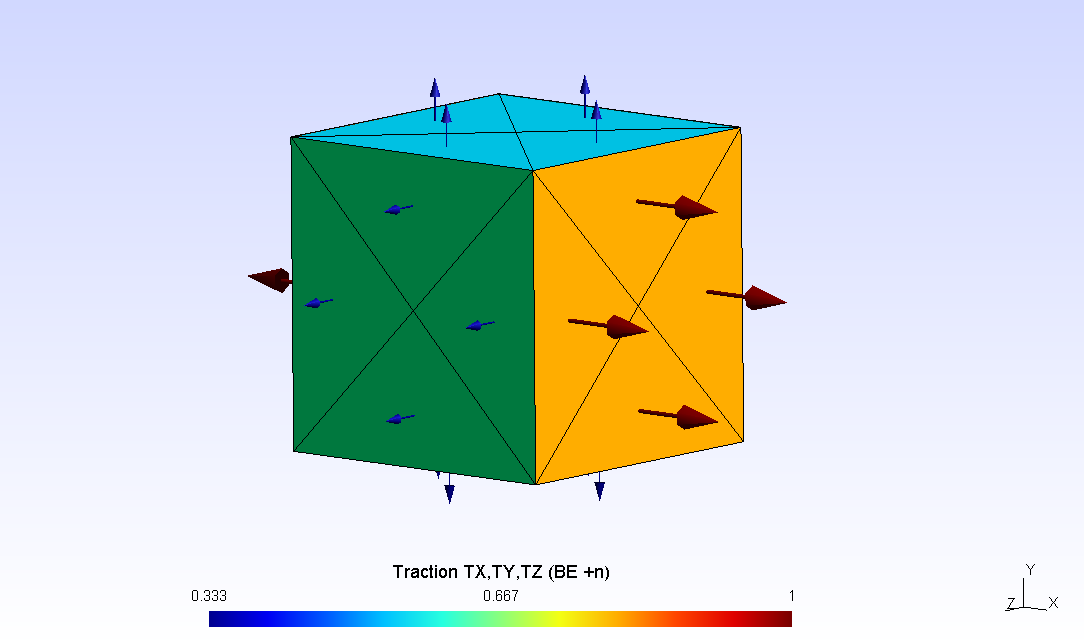
\includegraphics[scale = 0.5]{traction.png}
	\caption{File *.pos. Traction results.}
	\label{fig:traction}
\end{figure}

\begin{figure}
	\centering
	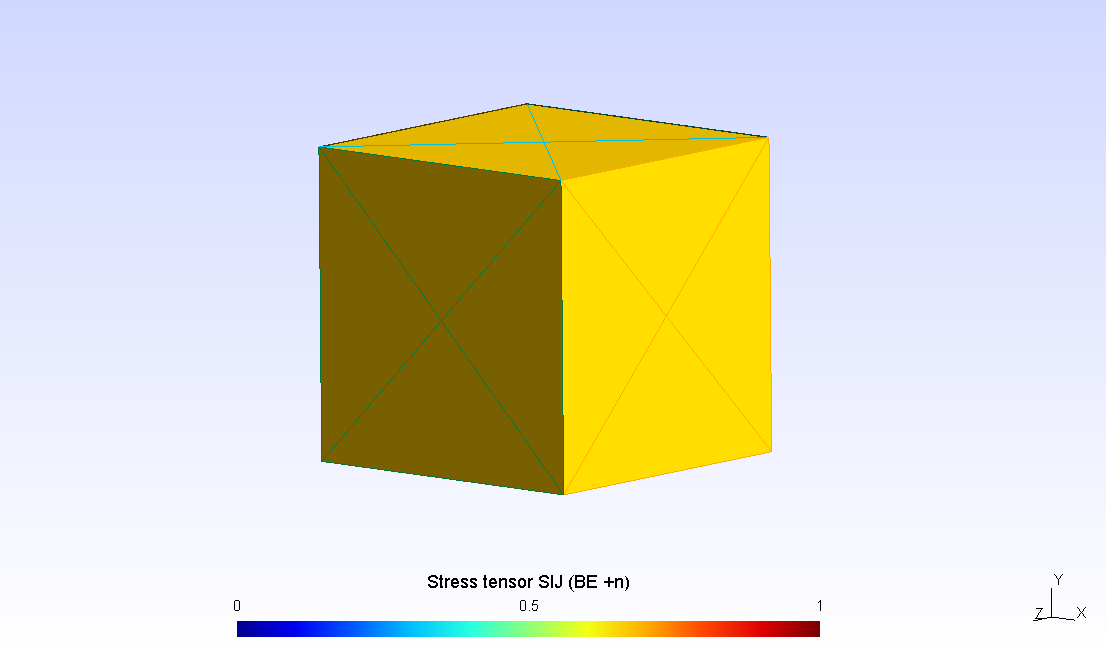
\includegraphics[scale = 0.5]{stress.png}
	\caption{File *.pos. Stress tensor results.}
	\label{fig:stress}
\end{figure}

\section{Results comparison}

The comparison between the analytical and numerical solutions for the third and fourth nodes are shown in Table \ref{tab:square_results}. It can be seen that the numerical solution is in perfect agreement with the analytical solution.

\begin{table}[h]
	\begin{center}
		\begin{tabular}{|*{4}{c}|}
			\hline
			Node & Variable & Analytical solution & Numerical solution \\
			\hline
			3 & $u_1$ & $0.8\overline{3}$ & 0.833333 \\
			\hline
			3 & $u_2$ & 0 & $0.311627\cdot 10^{-6}$ \\
			\hline
			3 & $t_1$ & 1 & 1.000000 \\
			\hline
			3 & $t_2$ & $0$ & 0.000000 \\
			\hline
			4 & $u_1$ & $0.8\overline{3}$ & 0.833333 \\
			\hline
			4 & $u_2$ & 0 & $-0.311627\cdot 10^{-6}$ \\
			\hline
			4 & $t_1$ & 1 & 1.000000 \\
			\hline
			4 & $t_2$ & $0$ & 0.000000 \\
			\hline
		\end{tabular}
	\end{center}
	\caption{Results comparison.}
	\label{tab:square_results}
\end{table}

\section{Modifications}

\subsection{Higher number of elements}

The process to obtain more elements for the mesh consists of specifying the element size in the *.geo file. For example, to obtain two elements per boundary it is enough to set the element size as 0.5.  

\subsection{Higher order elements}

The process to obtain higher order elements for the mesh consists of specifying the element order in the *.geo file. For example, to obtain cuadratic elements it is enough to set a "2" in the expression "SetOrder". 

\subsection{SBIE formulation}

It is worth mentioning that there is a discontinuity of displacement in the nodes shared by different boundaries. However, the reason for this discrepancy is due to the formulation by default of the solver. The best way to solve this issue is by means of a nodal collocation which can be specified with the following option in the input file: 

\begin{Verbatim}
[bem formulation over boundaries]
boundary 1: sbie
boundary 2: sbie
boundary 3: sbie
boundary 4: sbie
\end{Verbatim}

The results with this formulation are the following:

\begin{Verbatim}
0 0.0E+0 1 1 2 1 1 1 1 0.0E+0 0.0E+0 270.112E-18    0.000E+00    0.000E+0 -333.333E-3
0 0.0E+0 1 1 2 1 1 1 2 1.0E+0 0.0E+0 833.333E-03    0.000E+00    0.000E+0 -333.333E-3
0 0.0E+0 1 1 2 2 1 1 3 1.0E+0 0.0E+0 833.333E-03   96.375E-18    1.000E+0    0.000E+0
0 0.0E+0 1 1 2 2 1 1 4 1.0E+0 1.0E+0 833.333E-03  265.501E-18    1.000E+0    0.000E+0
0 0.0E+0 1 1 2 3 1 1 5 1.0E+0 1.0E+0 833.333E-03    0.000E+00    0.000E+0  333.333E-3
0 0.0E+0 1 1 2 3 1 1 6 0.0E+0 1.0E+0 241.448E-18    0.000E+00    0.000E+0  333.333E-3
0 0.0E+0 1 1 2 4 1 1 7 0.0E+0 1.0E+0   0.000E+00 -256.789E-18 -999.999E-3    0.000E+0
0 0.0E+0 1 1 2 4 1 1 8 0.0E+0 0.0E+0   0.000E+00  -25.547E-18 -999.999E-3    0.000E+0
\end{Verbatim}

\begin{thebibliography}{99}

	\bibitem{gmsh} C. Geuzaine and J.-F. Remacle, "Gmsh: a three-dimensional finite element mesh generator with built-in pre- and post-processing facilities." \emph{Int. J. Numer. Methods Eng.}, Volume 79, Issue 11, pages 1309--1331, (2009)
	
	\bibitem{gmshweb}  C. Geuzaine and J.-F. Remacle, "Gmsh." \url{http://gmsh.info/}
	
\end{thebibliography}


\end{document}
